\documentclass[12pt]{article}
\usepackage{amsmath}
\usepackage{graphicx}

\begin{document}
\begin{itemize}
    \item[Q1] Prove or disprove the following is not a regular language. If
        regular, write down its regular expression. Otherwise, prove it.
        \begin{itemize}
            \item[Q1.1] \{$O^n|n$ is a perfect number\}. A perfect number is a
                number whose square root is an integer.
            \item{\textbf{Answer:}} 
            \item[Q1.2] \{$a^nb^n|1 \leq n \leq 2021$\}
            \item[\textbf{Answer:}] n is a finite number and a finite automata
                can be used to model the language, with a total of $2*n$ states.
                Therefore, the language is regular and its regular expression is
                $(ab){1,2021}$, where the the strings accepted are the strings
                with $ab$ repeated between $1$ and $2021$ times.
            \item[Q1.3] \{$ww|w \exists \Sigma^*, \Sigma=\{0,1\}$\}
            \item[Q1.4] \{$0^m1^n| m \leq n$\}
            \item[\textbf{Answer:}] Memory is required to store the current
            number $m$ so that it can be compared to the number $n$ after
            accepting $m$ $0$s. Therefore, the language is not regular since
            memory is required.
        \end{itemize}
    \item[Q2] Prove the following statements.
        \begin{itemize}
            \item[Q2.1] $\bar L$ is regular if $L$ is regular.
            \item[\textbf{Answer:}] If we create an finite automata $A$ to
                represent $L$, then $\bar L$ can be represented by the same
                automata, with the accepting and non-accepting states flipped
                $B$. Any string $w$ is in $L(A)$ if and only if it is not in
                $L(B)$. Therefore, $B$ can be modeled with finite states and is
                regular.
            \item[Q2.2] $L \cap M$ is regular if $L$ and $M$ are regular.
            \item[\textbf{Answer:}] If we create a two finite automata that
                represent both $L$ and $M$, $A$ and $B$, we can group the two
                automata together and evaluate them in parallel. Then we can
                select accepting states that are pairs of all accepting states
                of $A$ and $B$. Finally, we model the union of $A$ and $B$ as a
                single automaton which can be represented with finite states.
                Therefore $L \cap M$ is regular.
        \end{itemize}
    \item[Q3] Given the DFA:
        \begin{figure}[h]
            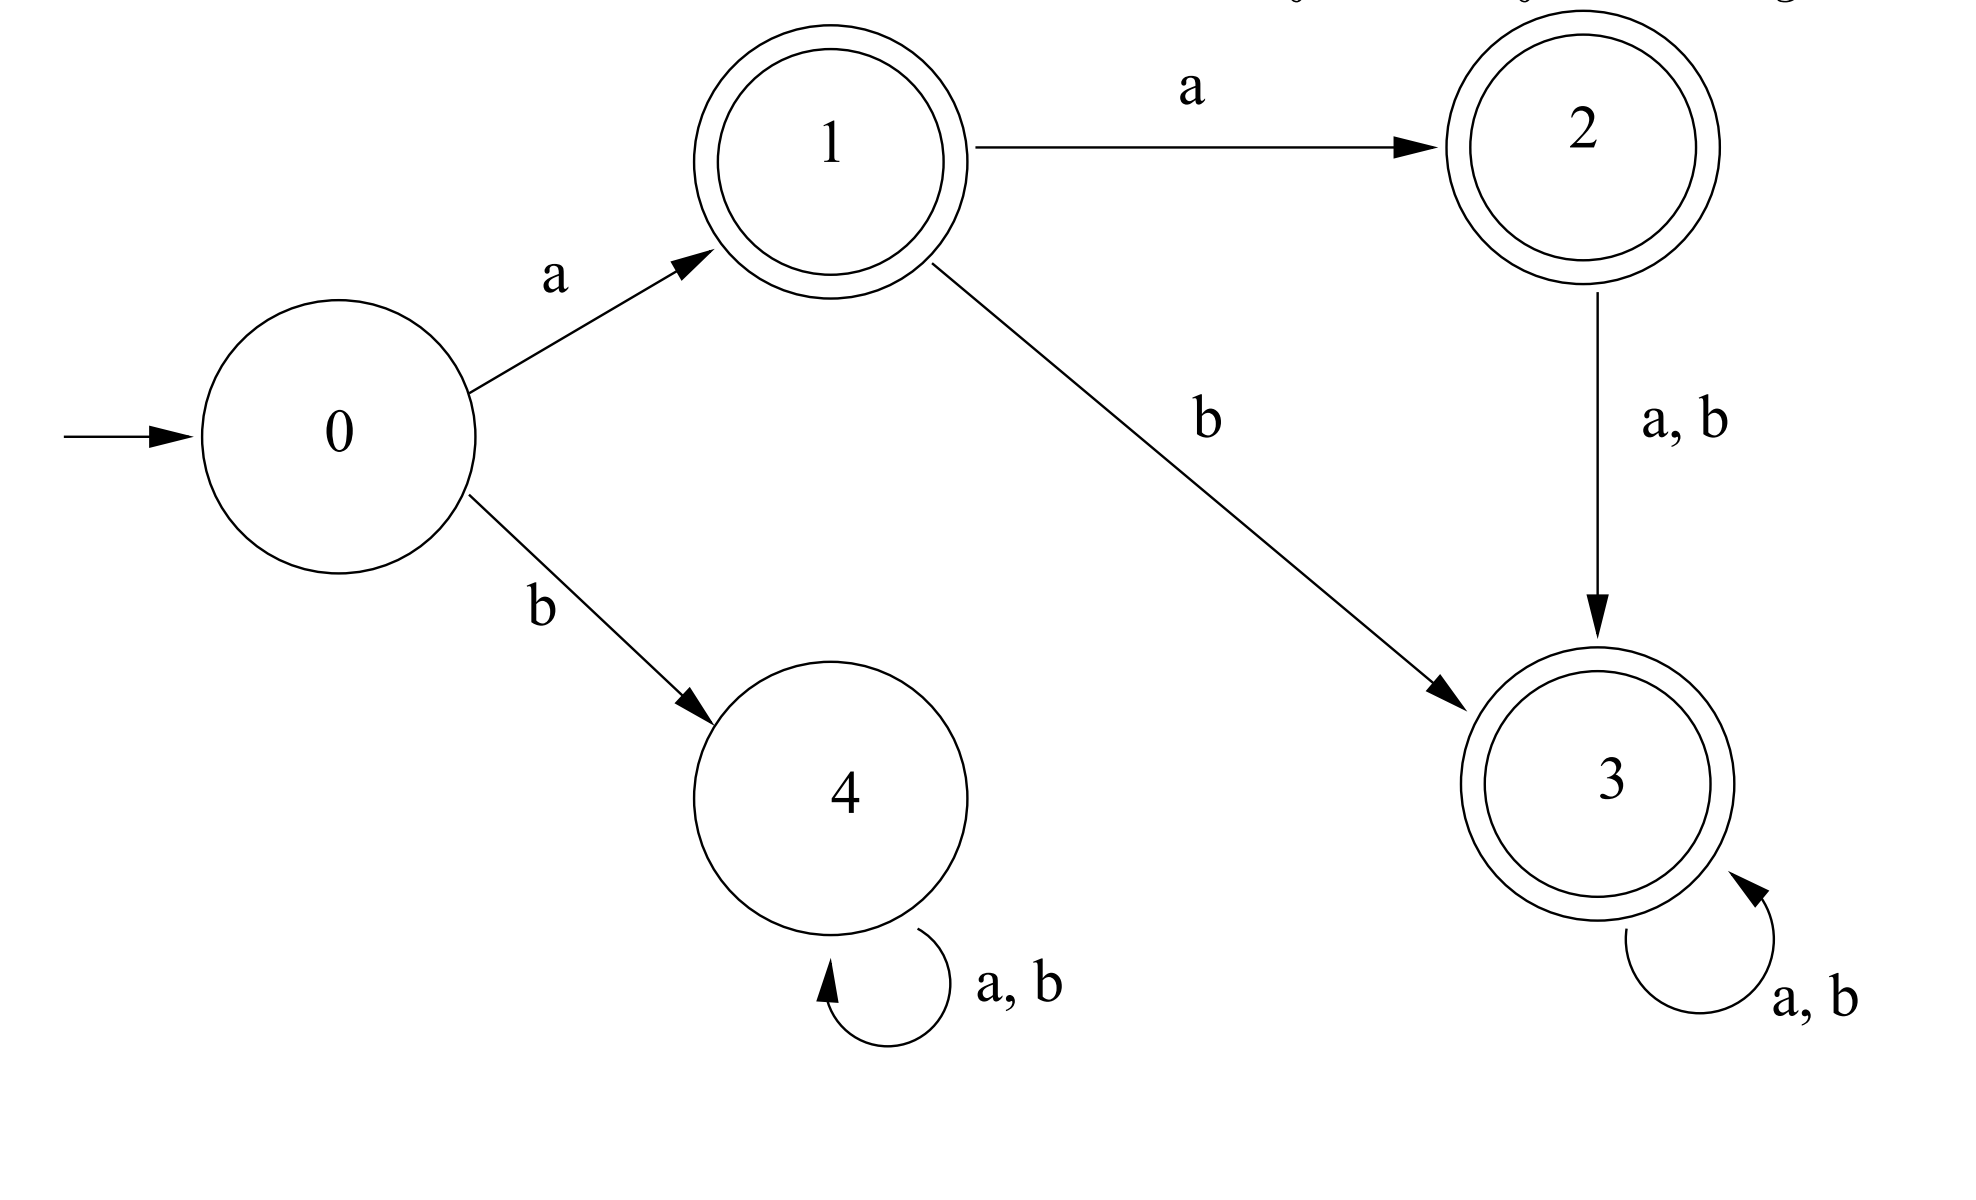
\includegraphics[width=0.8\textwidth]{assets/t2_q3.png}
        \end{figure}
        \begin{itemize}
            \item[Q3.1] What states are equivalent to state 3?
            \item[\textbf{Answer:}] State 2 is equivalent to state 3.
            \item[Q3.2] How many states are there in the minimized DFA?
            \item[\textbf{Answer:}] After combining states 2 and 3, there are 4
                states. However, the DFA can be further minimized. The combined
                state $\{2,3\}$ is equivalent to state $1$. Therefore, the final
                minimized DFA has 3 states: $[\{0\}, \{1,2,3\}, \{4\}]$. The
                language accepted by the DFA is any string $w$ in the language
                $L=\{a,b\}$ that starts with $a$.

        \end{itemize}
    \item[Q4] Which of the following conversion has the worst time complexity?
        \begin{itemize}
            \item[A] DFA to NFA
            \item[B] NFA to DFA
            \item[C] FA to RE
            \item[D] RE to FA
            \item[\textbf{Answer:}] C
        \end{itemize}
    \item[Q5] Given the context free grammar: $S \rightarrow
            aSbS|bSaS|\epsilon$. Is the grammar ambiguous? Yes/No
    \item[\textbf{Answer:}] Yes.
\end{itemize}
\end{document}
